\documentclass[12pt,a4paper]{report}
\usepackage[utf8]{inputenc}
\usepackage{amsmath}
\usepackage{amsfonts}
\usepackage{amssymb}
\usepackage{graphicx}
\usepackage{lmodern}
\usepackage{kpfonts}
\usepackage[left=2cm,right=2cm,top=2cm,bottom=2cm]{geometry}
\author{Team members \\{\normalsize Devan Patel, Kyle Koceski, and Daniel Fuentes}}
\title{Proposal \\ {\large Joseph Conway's Game of Life via Multithreading} }
\begin{document}
\maketitle
\newpage
\section{Team members}
\begin{enumerate}
\item Devan Patel - devanp92@ufl.edu
\item Daniel Fuentes - danielffuentes@ufl.edu
\item Kyle Koceski - kkoceski93@ufl.edu
\end{enumerate}
\section{Designated Submitter}
\paragraph{}
Devan Patel
\section{Project Overview}
\subparagraph{Implementation}
Our version of The Game of Life will be implemented in a server-client architecture (\ref{fig:csa}), providing a single game instance which can be controlled and played on multiple clients. Using this architecture, the calculation of the next iteration can be computed on multiple clients, as well as multiple threads on these clients. \\

On the server side, the game board will be maintained and updated according to commands from clients. The board will be constantly be transmitted to clients when changes are made. When the game is played, the server will also distribute the task of calculating the next iteration amongst the clients. These clients can then calculate the next iteration from the information they have, returning this information to the server. The server can then merge the calculations, distribute the board to the clients, and distribute tasks again for the next iteration. \\

On the client side, clients will be able to update the grid size and initial living cells and be able to play the game. Clients will then receive commands for calculating the next iteration. After these calculations are complete, the information is sent to the server for merging and the client waits for future information. 
\begin{figure}[ht!]
\centering
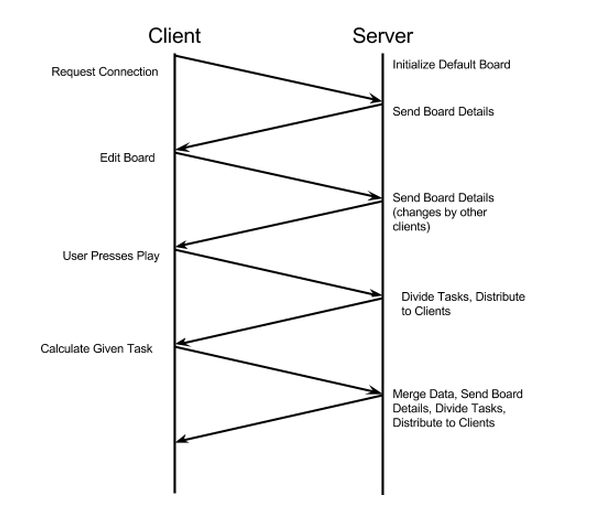
\includegraphics[width=90mm]{client_server_architecture.jpg}
\caption{Design overview of the client-server architecture}
\label{fig:csa}
\end{figure}

\subparagraph*{Design} 
The Game of Life will be implemented by managing the board as a list of alive cells. These alive cells can be evenly distributed to clients for calculation and determining whether nearby cells live or die. This calculation can be split further using multiple threads on each client managed by a ThreadPool. The ThreadPool comprises of multiple threads designated to determine if each cell will be alive or dead for a certain number of rows.
\section{How This Project Relates To Concurrent Programming}
\paragraph{}
In order to maintain a consistent state with multiple clients potentially modifying a board simultaneously, as well as handling the division and merging of multiple sets of data, proper concurrency techniques will need to be handled. \\

Alongside this, our implementation of the Game of Life will be multi-threaded; in the aforementioned it notes that there will be a selected thread dedicated to a certain number of rows (dependent on the grid size) which will determine which cells will be alive or dead in that iteration. \\

For each iteration, there will be a timed result which calculates the time difference between the start and end of each iteration. The timed results from the concurrent solution will be tested against a sequential version to produce comparisons in order to conclude if parallelism has produced a more efficient model than its sequential counterpart.
\section{Hardware and Software Used}
\paragraph{}
There will be no additional hardware required other than a multi-core laptop since our product is purely software based.
The software that we plan on using are as follows: 
\begin{itemize}
\item Backend - Java 1.7
\item Frontend - JSP 2.2, CSS, HTML5, and XML.
\item Testing - Apache JMeter
\end{itemize}
\end{document}